\subsection{欠点}

\paragraph{書き方が細かく定められている}
\begin{description}
\item 誤って一つでも消してしまうとエラーがでて動作しなくなってしまう.
\item emacs\_helpを例にする.emacs\_helpの内容は下のようになっている.
\\
\end{description}
\begin{quote}\begin{verbatim}
/Users/saki/.my_help% cat emacs_help.yml
---
:head:
- "emacsのキーバインド"
- "\n特殊キー操作"
- "  c-f, controlキーを押しながら    'f'"
- "  M-f, escキーを押した後一度離して'f'"
- "    操作の中断c-g, 操作の取り消し(Undo) c-x u"
:license:
- "     cc by Shigeto R. Nishitani, 2016"
:cursor:
  :opts:
    :short: "-c"
    :long: "--cursor"
    :desc: Cursor移動
  :cont:
  - c-f, move Forwrard,    前or右へ
  - c-b, move Backwrard,   後or左へ
  - c-a, go Ahead of line, 行頭へ
  - c-e, go End of line,   行末へ
  - c-n, move Next line,   次行へ
  - c-p, move Previous line, 前行へ
:page:
  :opts:
    :short: "-p"
    :long: "--ページ"
    :desc: Page移動
  :cont:
  - c-v, move Vertical,          次のページへ
  - M-v, move reversive Vertical,前のページへ
  - c-l, centerise Line,       現在行を中心に
  - M-<, move Top of file,    ファイルの先頭へ
  - M->, move Bottom of file, ファイルの最後尾へ
  
  (以下省略)
\end{verbatim}\end{quote}
\begin{description}
\item 1行目の\textbf{:head:}の後ろの\textbf{:}を消してみる.
\textbf{:}を消しただけで,メモを更新しようとすると
\end{description}
\begin{quote}\begin{verbatim}
/Users/saki/.my_help% emacs_help --edit
/System/Library/Frameworks/Ruby.framework/Versions/2.0/usr/lib/ruby/2.0.0/psych.rb:205:in `parse': (<unknown>): mapping values are not allowed in this context at line 8 column 9 (Psych::SyntaxError)
	from /System/Library/Frameworks/Ruby.framework/Versions/2.0/usr/lib/ruby/2.0.0/psych.rb:205:in `parse_stream'
	from /System/Library/Frameworks/Ruby.framework/Versions/2.0/usr/lib/ruby/2.0.0/psych.rb:153:in `parse'
	from /System/Library/Frameworks/Ruby.framework/Versions/2.0/usr/lib/ruby/2.0.0/psych.rb:129:in `load'
	from /Library/Ruby/Gems/2.0.0/gems/my_help-0.4.3/lib/specific_help.rb:17:in `initialize'
	from /Library/Ruby/Gems/2.0.0/gems/my_help-0.4.3/lib/specific_help.rb:12:in `new'
	from /Library/Ruby/Gems/2.0.0/gems/my_help-0.4.3/lib/specific_help.rb:12:in `run'
	from /Library/Ruby/Gems/2.0.0/gems/my_help-0.4.3/exe/emacs_help:4:in `<top (required)>'
	from /usr/bin/emacs_help:23:in `load'
	from /usr/bin/emacs_help:23:in `<main>'
\end{verbatim}\end{quote}
\begin{description}
\item このようになり,emacs\_helpが動かなくなってしまう.
使い慣れれば気づくことができるが,初心者ではエラーが見つけにくいと思われる.
\end{description}

\paragraph{my\_helpからlatexへの変換}
\begin{figure}[htbp]\begin{center}
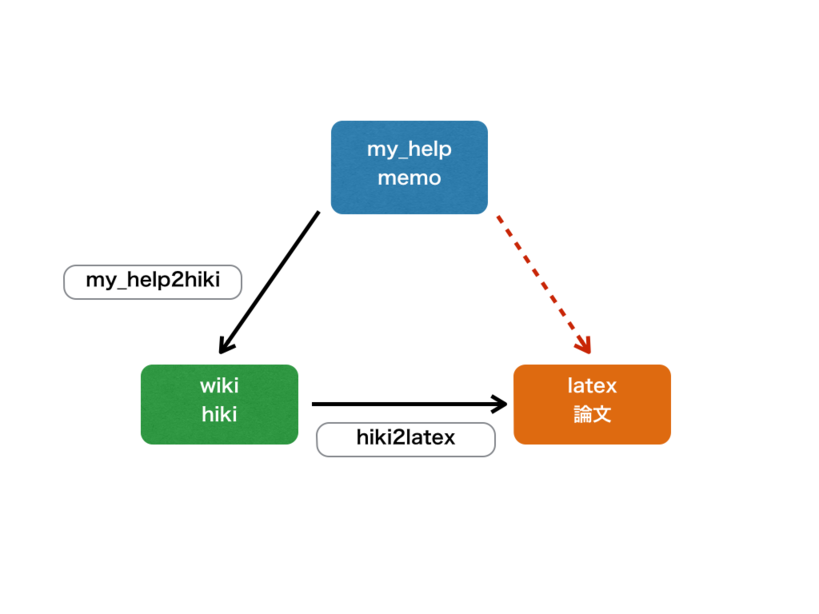
\includegraphics[width=6cm,bb=0 0 442 500]{my_help2hiki_saki.007.png}
\caption{my\_help2hikiによるmemo,hiki,latexの関係}
\label{default}\end{center}\end{figure}
\begin{description}
\item 上図からも分かるように,本研究のmy\_help2hikiでも,my\_helpからlatexへ変換するには
一度hikiに変換しなければlatexへ変換することができない.
\end{description}

\paragraph{コマンド}
\begin{description}
\item my\_helpからhikiへの変換,hikiからlatexへの変換の操作を行うコマンドの
二つを行わなければ全てのファイルを同じ内容にすることはできない.
\end{description}

\paragraph{西谷研究室の内部サイトへの表示}
\begin{description}
\item 西谷研究室には内部サイトがあり,研究室内で使うシステムのマニュアルなどが公開されている.
\item hiki形式への変換ができればwikiで表示することはできるようになるが,
my\_help2hikiのコマンドでwikiのページを作成しても,現段階では研究室内全員が見ることはできない.
\end{description}